\section{Introduction}

Intersections are among the most important bottlenecks in urban road networks. Conventional signal control allocates right-of-way by phases, but the fixed or semi-fixed structure of signal phases can leave unused capacity when traffic is sparse and can impose unnecessary stops when vehicles could otherwise coordinate safely. Connected and automated vehicles (CAVs) change the intersection-control problem because vehicles can share position, speed, route, and intention information with a roadside controller or with each other. In a fully connected and automated setting, the intersection can be managed as a space-time resource allocation problem rather than as a fixed signal cycle.

Autonomous intersection management (AIM) was introduced as a reservation-based multiagent control problem in which vehicles request access to space-time regions of an intersection \cite{dresner2008multiagent}. Later work developed graph-based models that divide an intersection into conflict zones and verify collision-free and deadlock-free passing orders \cite{lin2019graph}. The connection to job-shop scheduling is natural: vehicles are jobs, conflict zones are machines or resources, and the traversal of a conflict zone is an operation. Huang et al. recently used this mapping to transform graph-based AIM into a constrained job-shop scheduling problem (JSSP) and trained a centralized intersection manager with proximal policy optimization (PPO) \cite{huang2023reinforcement}.

This paper develops a formulation-level extension of that direction. The main idea is that real traffic is heterogeneous. A passenger car, a bus, a truck, and an emergency vehicle should not necessarily be treated as identical jobs with identical delay costs. Buses may represent larger person-delay, trucks may require longer conflict-zone occupation and safety headway, and emergency vehicles may require hard or near-hard priority. At the same time, priority cannot relax physical safety: no vehicle class may violate conflict-zone capacity, trajectory order, same-lane order, blocking feasibility, or deadlock constraints.

The proposed contribution is a priority-aware constrained JSSP formulation for single-intersection AIM. Each vehicle is represented by an arrival or release time, a predicted trajectory through conflict zones, a class label, physical traversal parameters, and a priority weight. The scheduling objective minimizes weighted delay with an optional fairness term. The framework is designed for online receding-horizon execution, where the controller repeatedly predicts near-future vehicle arrivals, constructs a finite constrained-JSSP instance, schedules feasible operations, executes only near-term decisions, and re-plans as the traffic stream changes.

The paper makes the following formulation contributions:
\begin{itemize}
    \item It defines a priority-aware constrained-JSSP model for heterogeneous CAV intersection scheduling.
    \item It separates priority from safety: priority affects the objective or emergency constraints, while safety is enforced by resource, ordering, blocking, and deadlock constraints.
    \item It gives a receding-horizon scheduling architecture that can use kinematic or learned prediction of arrival and conflict-zone occupation times.
    \item It specifies non-learning and learning-based baselines for a future implementation, including FCFS, greedy, priority-greedy, deadlock-aware greedy, small-instance optimization, and PPO/GNN dispatching.
\end{itemize}

Fig.~\ref{fig:framework} summarizes the intended framework. The figure is included from the existing repository material and should be replaced by a publication-ready diagram before submission.

\begin{figure}[t]
    \centering
    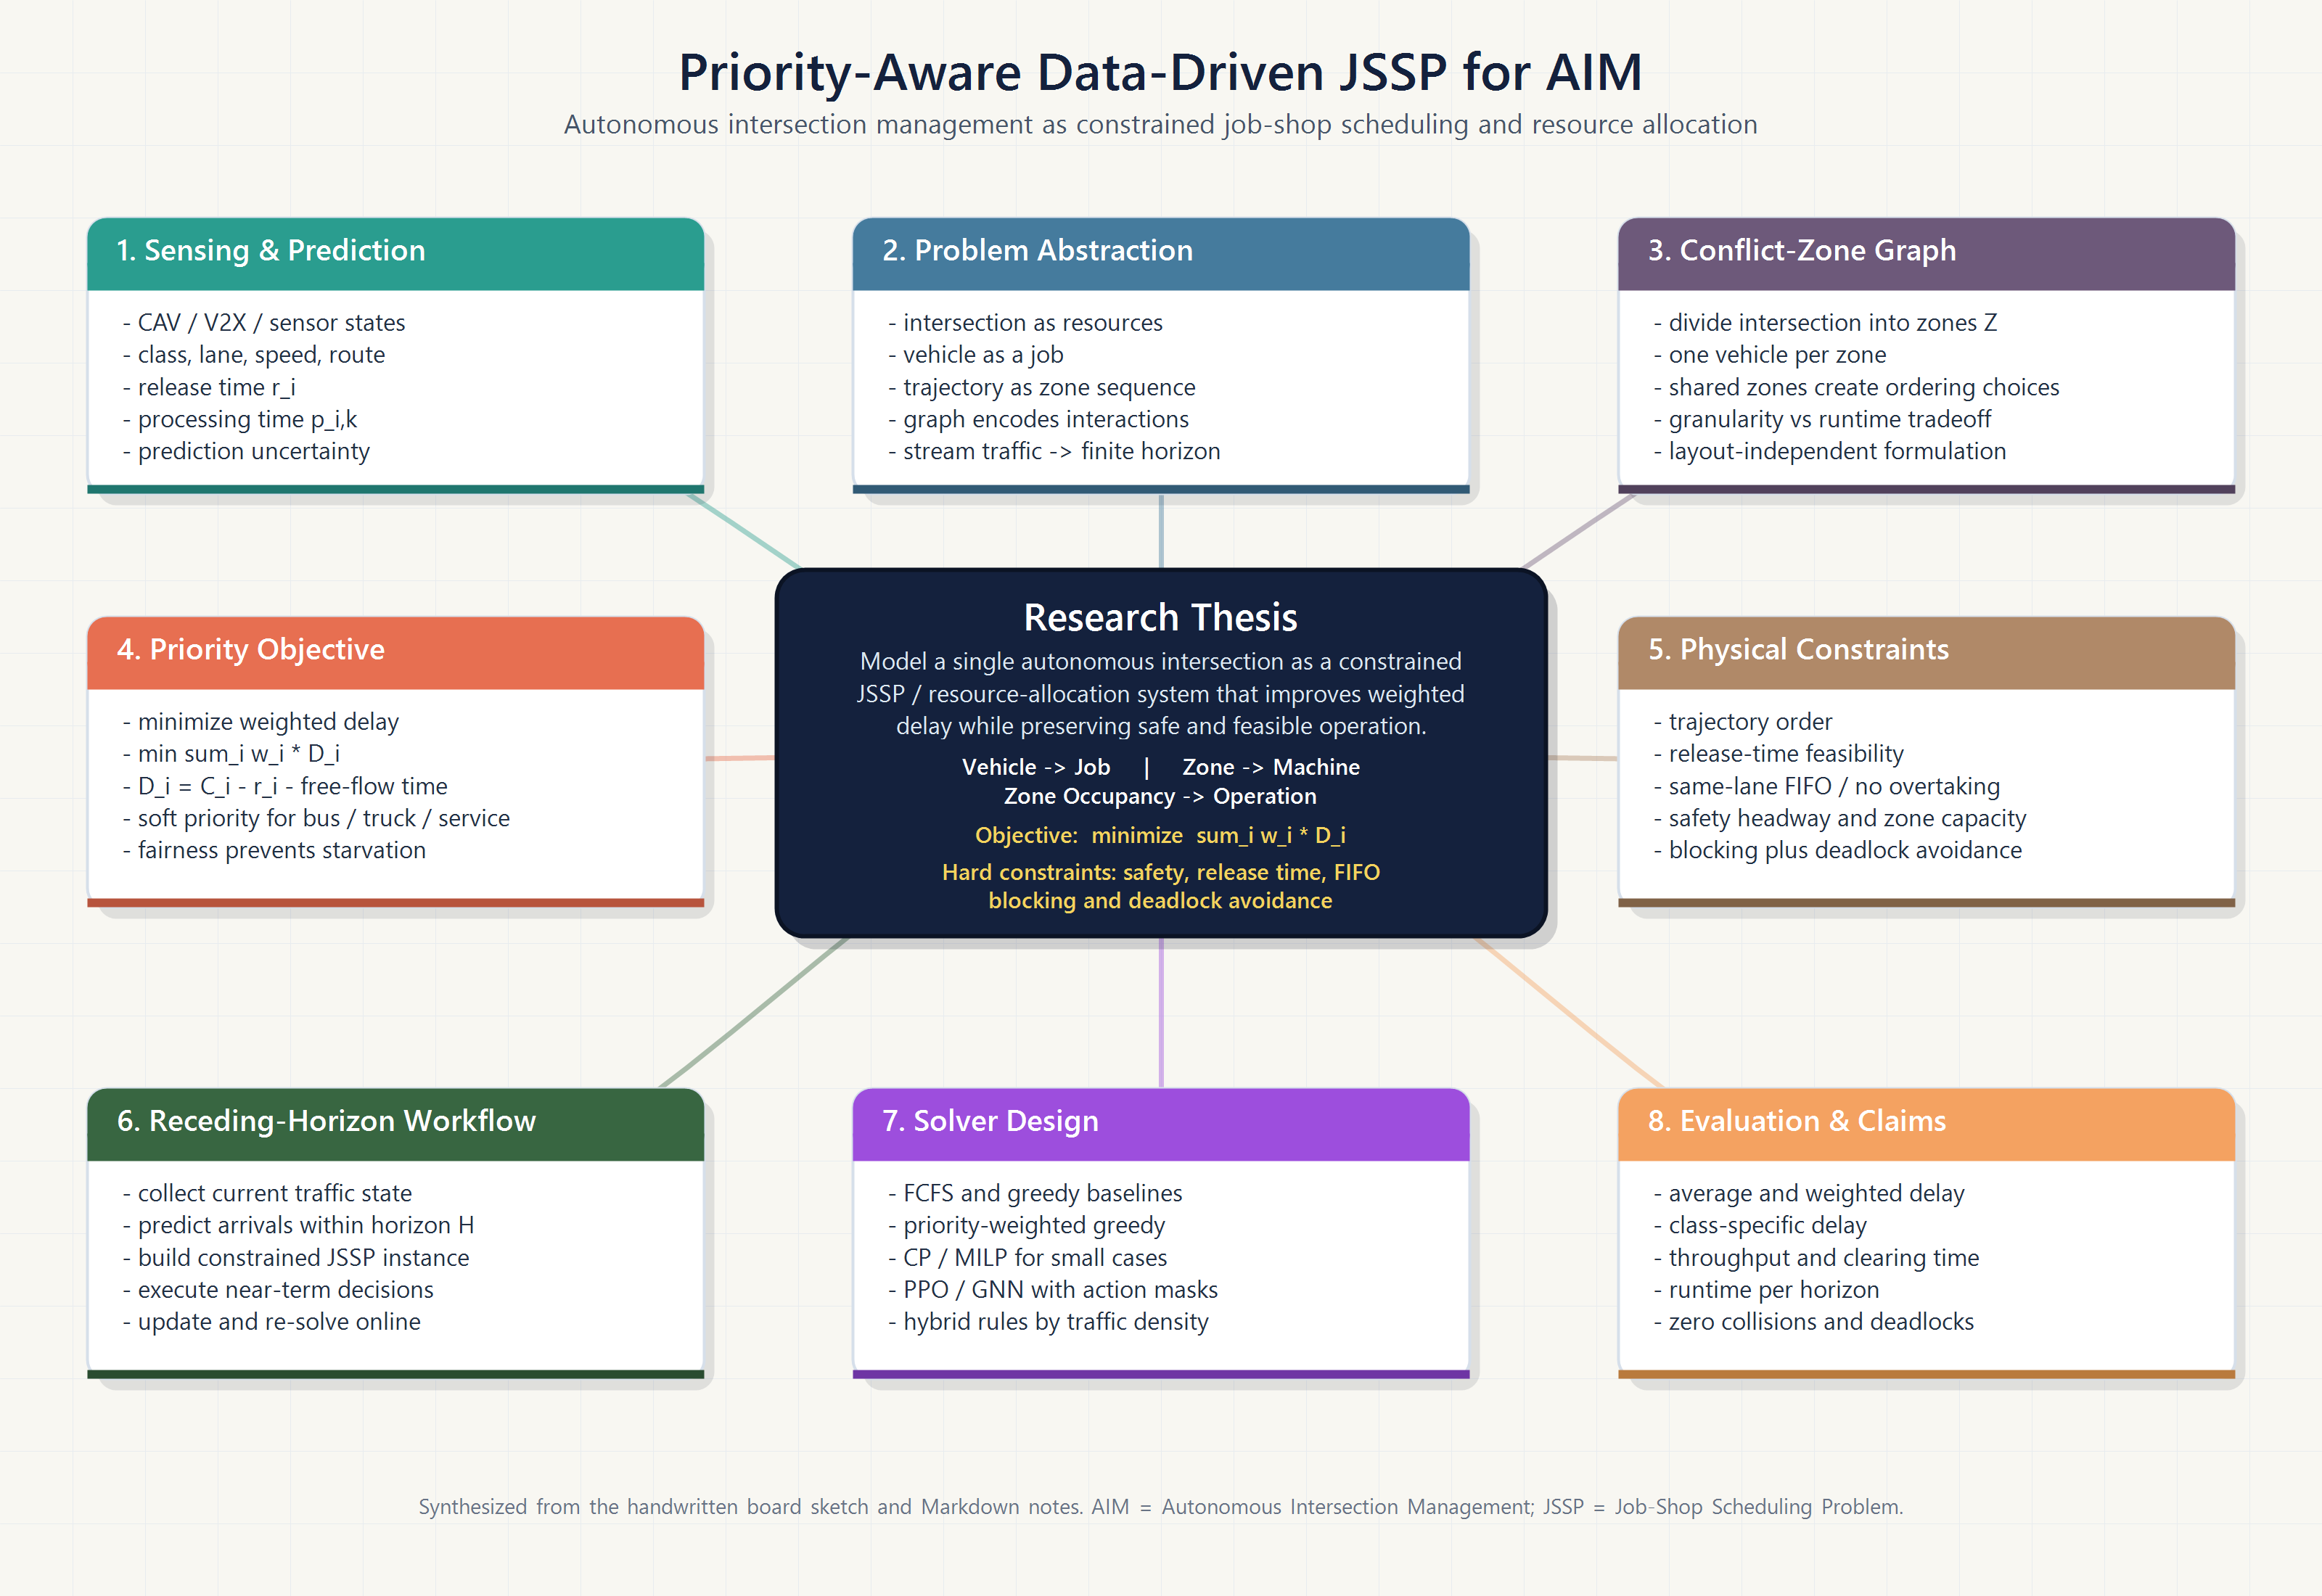
\includegraphics[width=\linewidth]{../../Pic/PriorityAwareJSSPAIMMindMap.png}
    \caption{Conceptual framework for priority-aware data-driven JSSP-based autonomous intersection management.}
    \label{fig:framework}
\end{figure}

